% this sections containes all the references for each section : 

% 1. group articles by field 




\section{benchmarking}

this is \cite{arcuri_practical_2011}

difference tests  \cite{sonnenwald2003evaluating}
%further references 
\cite{lilja2005measuring}
\cite{bukh1992art}
%%%%%%%%%%%%%%%%%

list of benchmarks \cite{van_der_kouwe_benchmarking_2018}:
\begin{itemize}
    \item  Not evaluating potential performance degradation
    \item  Benchmark subsetting without proper justification
    \item  Selective data set hiding deficiencies
    \item  Microbenchmarks representing overall performance
    \item  Throughput degraded by x\% => overhead is \%
    \item  Creative overhead accounting
    \item  No indication of significance of data
    \item  Incorrect averaging across benchmark scores
    \item  Benchmarking of simplified simulated system
    \item  Inappropriate and misleading benchmarks
    \item  Same dataset for calibration and validation
    \item  No proper baseline
    \item  Only evaluate against yourself
    \item  Unfair benchmarking of competitors
    \item  Not all contributions evaluated
    \item  Only measure runtime overhead
    \item  False positives/negatives not tested
    \item  Elements of solution not tested incrementally
    \item  Missing platform specification
    \item  Missing software versions
    \item  Subbenchmarks not listed
    \item  Relative numbers only
\end{itemize}
% further references 
\cite{mytkowicz2009producing}
%%%%%%%%%% 

startup performance vs steady performance \cite{buytaert_statistically_nodate}


%%%%% ** reasons behind the energy variation ****

simgrid simulation of power consumption of parallel aplication using simgrid \cite{heinrich2017predicting}

impact of manifacturing process on the energy variation \cite{coles2014comparing}

different energy consumption between identical processers [ idle and hight load ]\cite{von2016variations}

the temperature is the main raison a high energy variation \cite{wang2018potential}

external factors are impact on the energy variation \cite{mukherjee2009spatio}

the place of the server in the room doesn't affect the energy variation \cite{diouri2013your}

comparaison of three measuring tools and they did exhebit 10\% variation each time \cite{inadomi2015analyzing}

%%****** mitigating the energy variation ******
low-cost scalable variation-aware algorithm \cite{inadomi2015analyzing}

reducing the energy variation by disabling turbo boost \cite{acun2016variation}

reducing the energy consumption in parallel systems \cite{chasapis2016runtime}

\cite{marathe2017empirical}


%\\\ https://www.cpubenchmark.net/compare/Intel-i7-12700KF-vs-Intel-i7-12700F/4608vs4692 | hardware benchmarking 
\section{energy consumption}

to be able to reduce the energy cost of running programs we should first be able to estame this energy consumption.
many studies have been conducted to estimate a such energy consumption. that varries from static analysis of the source code to enfere it's energy consumption like \citeauthor{pereira_helping_2017} where they provided a tool to highlight the most energy consuming parts of the code \cite{pereira_helping_2017}.the main advantage of this apporach is to be able to estimate the energy consumption of a program without running it. however. unlike the conplexity of programs, the energy consumption is highly related the execusion environment. Therefor, Static analysis might not represent the real behaviour of the same program when it is run in the production environment.
To treat the problem of representativeness, many researchers tend to measure the energy consumption of the programs while they are running them. Hence we will get more accurate results.
there is a variety of tools to measure such energy, and they cover a large spectrium of usage depends on how \textbf{accurate} and \textbf{pricise} those results are needed to be in tone hand, and the price that practinoners are ready to pay for a such accuray/pricision.
Below we will present some tools that are well known in the literature and discuss their main advantages / drawbacks for our case.
\subsection{hardware tools}

% TODO Add : diagram of the possible point where we can measure the energy 

% depends on the scientific usage there are two apporaches :
% 1. extern one or independent : when the most of researchs are using
% the benifits of this is the simplicity of instalation however we pay the price either with a lack of temporal resolution ( low frequency ) or the spatial granularity
% ( most of them measure the energy consumption of the whole machine )
% 2. dedicated one , they are based on the instrumentation of some parts of the computer , however they have a high cost and they are defficult to scale since they require an instrumentation of the execusion environment.
according to \citeauthor{hackenberg2014hdeem} there are four main creterions to evaluate an energy measurement tool \cite{hackenberg2014hdeem}
\begin{itemize}
    \item \em{spatial granularity}: the more specific the target of monitoring we are able to measure, the more efficient we can do optimization since we will know what causes the pitfalls of the energy consumption.
    \item \em{temporal granularity}: same as spatial granularity, temporal granularity helps us to identif the sequence of code that need to be optimized.
    \item \em{scalability}: this is mainly related to the cost of the tools and the ease of their integration for our system.
    \item  \em{accuracy}:to elimanate extra hazards and get more representative measurement.
\end{itemize}

We believe that accuracy can be extracted from those creterions since it is a result of the combaination of the two first ones. therefore, we will focus more on the first 3 creterions from later on.
In the follwong section we will discuss some of the well known tools that are used in literature.


Nowdays, most of the high performance computing systems (HPC) implements a tool to report the energy consumption of the nodes for the sake of monitoring and administration. Those tools are mainly integrated withing the power suply units (PSU) or the power distributuin units (PDU). then , they provide an interface and a log to follow the history of the energy consumption. Despite their scalability and ease of integration. such tools lack both in spatial and temporal granularity since they monitor the whole energy of the nodes, and most of the times they have a very low sampling frequency. most of those tools are provided directly by the manufacturers. such as \em{IBM EnergyScale technology} \cite{mccreary2007energyscale} \cite{caldeira2014ibm} \cite{caldeiraibm} or \em{Dell poweredge} \cite{lovicott2009thermal}, MEGware Cluststafe \cite{breitbart2015case}
As we said earlier the true purpose of those tools is more monitoring than analysing the energy consumption.
%% add something to link with wattsup pro 
WattsUp Pro, is a device that can be installed  between the  powerer source of the machine and the system under test. it allows a sampling frequency up to 1Hz and has a internal memory to store a wide variety of data, such as the maximum voltage, current.. etc that later can be exported via USB port for personal usage or lined to some graph programs like Logger Pro or LabQuest.The main advantage of this tool is the ability to monitor the energy consumption from a different device which will reduce the risk of interference with the energy consumption of the test % a revoir 
\cite{hirst2013watts}

despite his high temporal granularity  , wattsup pro lacks in term of spatial granularity since it monitors the energy consumption of the whole system.
To have a finer granularity we need to isolate the energy consumption of each component.
.
For this we will need more intrusive tools such.

%% THIS IS FOR GPU %%% 
% GPU TESLA \cite{burtscher2014measuring}

% NVML\cite{fahad2019comparative}
%%%% 

PowerMon and its upgradded version powerMon2 \cite{bedard2010powermon} are based on an microcontroler chip that can monitor up to 6 channel ( 8 for powermon2) simultanetly. therefore we are able to monitor the powerconsumption of 4 devices at the same time. the frequency sample of this tool is up to 50Hz with an accuracy of 1.2\%. Powermore2 comes with smaller size that can fit within 3.5 inches rack drive.

PowerInsight \cite{laros2013powerinsight} is another finegrained measurement tool that is based on an ARM bagelbone processor \cite{coley2012beaglebone} which is able to measure up to 30 channel simultanetly with a frequency of 1KHz per channel.

on the other hand GreenMiner \cite{hindle2014greenminer}, %%i dont think that  mobile measurement will be relevent for my case 

powerpack \cite{ge2009powerpack} in the other hand is an api that synchronizes the data gathered from other monitoring tools such as Watt’s Up Pro, NI and RadioShack pro and the lines of code %% maybe remove this one from the list because it is not well known.

other monitor tools have been relized by the manufactures such as IBM Power executive \cite{koomey2011growth} which allows their customer to monitor the power consumption and thermal behaviour of the of BladeCenter systems in the datacenter.



%% TODO : add diagram where the distribution of the energy consumption is more related to the CPU rather than other tools - u can cite the tools dedicated to the GPU since it is is included in the software aggregators ? power api, pythoules ...etc 

as we see in % two diagrams one for research the other one for power usage 
The CPU is the part responsible of the most energy consumption of softwares. hence the finner we go to measure this energy consumption the better it is for our work.
Fortunately, Intel and later AMD proposed a tool that estimate the power consumption of different part of the CPI based on counter performances. RAPL (RUnning Average Power Limit) \cite{hackenberg2013power} \cite{hackenberg2015energy} is a set of registers that was introduced by intel in their CPU since Sandy bridge generation, and later it was fllowed by AMD since Family 17h Zen.
It is capable of monitoring different components of CPU , such as DRAM, Cores , and the integrated GPU for desktop processors.

%% TODO :ADD figure of RAPL + references 

The advanage of a such apporach is that the absence of any intrusive measurement tools. further more they have a high temporal granurality with a sampling frequency up to 1KHz \cite{ilsche_power_2015}.

with similar approach we can find NVIDIA reporting tools such as GPU TESLA \cite{burtscher2014measuring} and the NVML library \cite{fahad2019comparative}


\subsection{software tools}
Now that we got our hands on a precise tools that allows us to monitor

powerapi \cite{colmant2018next}

smartwatts formula \cite{fieni2020smartwatts}

Wattwatcher \cite{lebeane2015watt}

joulemeter \cite{kothari2009joulemeter}\cite{jagroep2017energy}

jrapl \cite{guimaraes2016some} \cite{liu2015data}

joulinar \cite{islam2016measuring} \cite{noureddine2016jolinar}

jalen \cite{noureddine2015monitoring}

selfwatts \cite{fieni2021selfwatts}

powerjoular \cite{noureddine2022powerjoular}
\subsection{hybrid tools}
% split hardware tools into extern and embeded tools 


\section{programming languages and performances}
\subsection{energy}


energy comparaison of programming languages in the game benchmark by debian \cite{pereira2017energy}

toward green ranking \cite{couto2017towards}

java vs kotlin in web performances \cite{bujnowski2020java}

rosetta code \cite{nanz2015comparative} \cite{mirowski2020rosetta}

network energy comparaison \cite{balasubramanian2009energy}

Aequitas \cite{ribic2016aequitas}

vm placement \cite{mishra2018energy}

\citeauthor{mishra2018energy}

static cost of Vms \cite{kurpicz2016much}



carbon footprint of training neural network \cite{strubell2019energy}

SPELL, the energy leaks detector tool \cite{pereira2017helping}

impact of energy profiling on software \cite{jagroep2017energy}

impact of maintability on software energy evolution \cite{calero2021does}

\subsection{jvm}

java vs python \cite{destefanis_statistical_2016}

hotspot vs J9 \cite{oi2011power} - same but for big querries \cite{chiba2018towards}

constant overheat of the jvm \cite{lafond2006energy}

infer the energy cost based on the byte code instructions \cite{ma2017biogeography}

java collection energy footprint  \cite{pinto2016comprehensive} \cite{fernandes2017assisting}

java classes energy footprint \cite{hasan2016energy}

framework to reduce java collections \cite{manotas2014seeds}

energy consumption of java dev tools \cite{baskar2013experimental}

Microbenchmarks on jvm \cite{longo2019reducing} \cite{baskar2013experimental}

android automatic refactoring to reduce energy consumption \cite{banerjee2016automated} \cite{rodriguez2017reducing}

java vs native c in android \cite{corral2014method}





\subsection{benchmarking}

NAS \cite{bailey_nas_nodate}



statistics \cite{he_statistics-based_2019}

benchmark crimes \cite{van_der_kouwe_benchmarking_2018}

microservices \cite{grambow_benchmarking_2020}

impact of webservers on web applications energy \cite{manotas_investigating_2013}



\subsection{frameworks}

impact of website implemenation on energy consumption \cite{philippot_characterization_2014} \cite{manotas2013investigating}

PHP \cite{benmoussa_new_2019} \cite{das_comparison_2016}

simulation of web cache \cite{cardenas_performance_2005}

java spring analysis \cite{gajewski_analysis_2019}

performance \cite{mishra2021web}



cross compiler bencharking \cite{yet2016cross}

\subsection{python}

webframeworks on python \cite{pankiv_concurrent_nodate}

hope library \cite{akeret_hope_2015}

bytecode effect \cite{ben_asher_effect_2009}

numba \cite{crist_dask_2016}

intel python \cite{li_boosting_2016}

python 2 vs 3 \cite{modzelewski_pyston_2020}

python runtime performances \cite{redondo_comprehensive_2015} \cite{murri_performance_2013}

static vs dynamic languages \cite{pang_what_nodate}

concurent benchmark framework \cite{pankiv2019concurrent}



\subsection{grpc}

defintion \cite{wang1993grpc}

comparaison \cite{chamas2017comparing}

emprical study \cite{de2021empirical}



\section{Conclusion}
As we have seen in the state of the art, many methodes have been proposed to reduce the energy footprint of the the ICT,which they can be applied in deffirent parts of the lifecycle of the program, from consumption to the execution. Furthermore, the execution phase took attention of many researchers because it's the part where the most energy is consumed. This thesis will focus on that aspect as well. However, unlike the most work that have been done on the hardware aspect, we will target the software impact on this energy, starting from the choice of the programming language up to how to tune some features of a frameworks in order to make the software consumes less energy.To do so we use the emprical apporach due to it's concinstency for the moment.Unlike the perfromance which essentialy related to the complexity of the algorithm, the energy consumption is more impacted by the hardware.
Therefore, to optimize the enrgy consumption we choose a spiral methode. based on 3 phases:
\begin{enumerate}
    \item execute the code
    \item measure the program
    \item infere the guidelines
\end{enumerate}


\begin{figure}[!hbt]
    \center{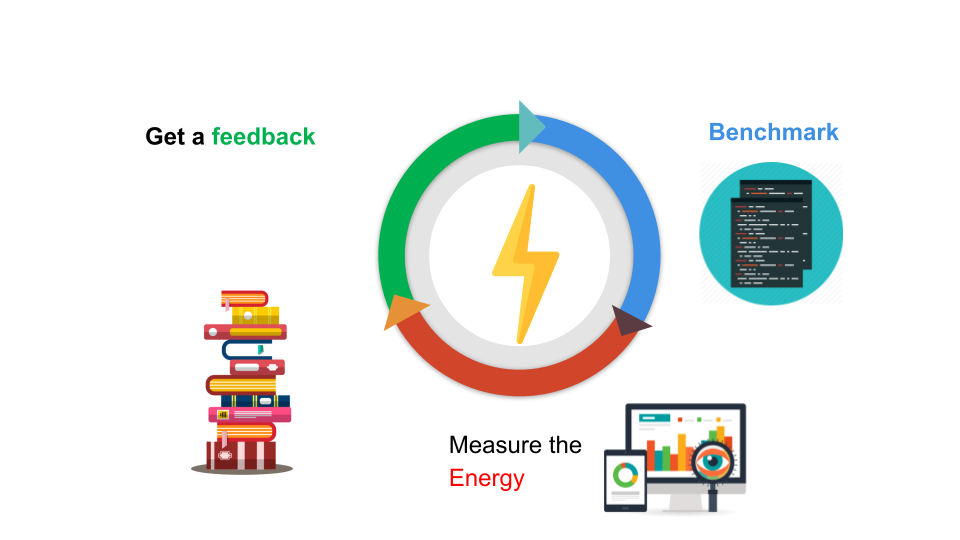
\includegraphics[scale=0.3]{images/greenbenchmarkcycle}}
    \caption{the spiral methode of energy optimization }\label{fig:spirals}
\end{figure}
the aim of this work is to present a set of guidelines to create a benchmarking system to to measure the energy consumption of different programs.
After that, we will use this system to compare the energy consumption of different programming languages. We will extend the work of \citeauthor{pereira2017energy} to a closer distance to production environment by comparing a set of usecases. starting by GRPC framework, and a set of Web Framewroks. Finally we will discuss the impact of the execution environment on the energy consumption of two of the most famous programming languages JAVA and Python. and present how can tunning the Virtual Machine can reduce the energy consumption.

